\documentclass[aspectratio=169,unicode,dvipdfmx,14pt]{beamer}


\usepackage{url}
\usepackage{bm}
\usepackage{amsmath}
\usepackage{amssymb}
\usepackage{mathtools}
\usepackage{graphicx}
\usepackage[absolute,overlay]{textpos}
\usepackage{hyperref}
\usepackage{listings}
\usepackage{changepage}
\usepackage{lipsum}


\usefonttheme[onlymath]{serif}

\DeclareMathOperator*{\argmax}{argmax}

\DeclarePairedDelimiterX{\infdivx}[2]{(}{)}{%
  #1\;\delimsize\|\;#2%
}
\newcommand{\infdiv}{D_{\scriptsize \mbox{KL}}\infdivx}
\DeclarePairedDelimiter{\norm}{\lVert}{\rVert}

\hypersetup{
	setpagesize=false,
	bookmarksnumbered=true,%
	bookmarksopen=true,%
	colorlinks=true,%
	linkcolor=blue,
	citecolor=red,
}

\newcommand\FontMath{\fontsize{10}{12}\selectfont}
\renewcommand{\baselinestretch}{1.3}
\renewcommand{\familydefault}{\sfdefault}
\renewcommand{\kanjifamilydefault}{\gtdefault}
\usepackage[deluxe, expert]{otf}

\setbeamertemplate{navigation symbols}{}
\setbeamertemplate{footline}[frame number]
\setbeamerfont{footline}{size={\fontsize{15}{15}}}

\setbeamerfont{author}{size=\Large}
\setbeamerfont{institute}{size=\normalsize\itshape}
\setbeamerfont{title}{size=\huge}
\setbeamerfont{subtitle}{size=\LARGE\normalfont\slshape}


\title{ \\多項分布を使った\\ベイズ的モデリング}
\author{\texorpdfstring{正田 備也\newline\href{mailto:masada@rikkyo.ac.jp}{masada@rikkyo.ac.jp}}{正田 備也}}
\date{}

\begin{document}

\begin{frame}
\titlepage
\end{frame}

\section{多項分布の復習}

\begin{frame}\frametitle{Contents}
\Large \tableofcontents[currentsection]
\end{frame}

\begin{frame}{カテゴリカル分布}
\begin{itemize}
\item $\mbox{V}=\{\mbox{v}_1,\ldots,\mbox{v}_W\}$を$W$種類のアイテムの集合とする
\begin{itemize}
\item[例1.] サイコロの目($W=6$)
\item[例2.] 自然言語の語彙($W=\mbox{数千〜数十万}$)
\end{itemize}
\item カテゴリカル分布は$\mbox{V}$上に定義された離散確率分布
\item パラメータは$\bm{\phi}=(\phi_1,\ldots,\phi_W)$
\begin{itemize}
\item アイテム$\mbox{v}_w$が出現する確率$\phi_w$
\item $\sum_{w=1}^W \phi_w = 1$を満たす
\item 自由度は$W-1$
\item[] \ 
\item[] \ 
\end{itemize}
\end{itemize}
\begin{textblock*}{0.5\linewidth}(230pt, 150pt)
    \centering
    \includegraphics[width=0.7\linewidth]{dice_bar_chart.png}
\end{textblock*}
\end{frame}


\begin{frame}{多項分布 multinomial distribution}
\begin{itemize}
\item カテゴリカル分布は、1回の試行のモデリングに使う
\item 複数回の独立な試行のモデリングには、多項分布を使う
\item 計$n$回の試行のうち各アイテムが何回ずつ出現するか、その可能なすべての場合に確率を割り振る確率分布が多項分布
\begin{itemize}
\item 次のスライド参照
\end{itemize}
\item パラメータは$n$と$\bm{\phi}=(\phi_1,\ldots,\phi_W)$
\begin{itemize}
\item 試行の回数$n$(観測データから決まる)
\item アイテム$\mbox{v}_w$の出現確率$\phi_w$($\sum_w \phi_w = 1$を満たす)
\item $\sum_w \phi_w=1$が満たされるので、自由度は$W-1$
\end{itemize}
\end{itemize}
\end{frame}

\begin{frame}{多項分布はどのような集合の上に定義されるか}
\begin{itemize}
\item 多項分布は``計$n$回の試行のうち各アイテムが何回ずつ出現するかの、可能な全ての場合の集合''の上に定義される
\item $W$種類のアイテムから重複を許して$n$個を選ぶすべての場合にわたって確率を合計すると、1になる
\begin{itemize}
\item $W$種類のアイテムから重複を許して$n$個を選ぶ場合の数は?
\item $n$個の「◯」と$W-1$個の「|」(仕切り)を並べる場合の数と同じ
\item[例.] 「◯ ◯ || ◯ | ◯ ◯ ◯ 」は、$n=6$で、$\mbox{v}_1$が2回、$\mbox{v}_2$が0回、$\mbox{v}_3$が1回、$\mbox{v}_4$が3回、それぞれ出現する場合を表す
\end{itemize}
\end{itemize}
\end{frame}

\begin{frame}{多項分布の確率質量関数}
\begin{itemize}
\item アイテム$\mbox{v}_w$の出現回数を$c_w$と書くことにする
\item 総試行回数を$n$とすると、$\sum_w c_w = n$が成り立つ
\item このとき、多項分布の確率質量関数pmfは以下ように書ける
\begin{align}
p((c_1,\ldots,c_W);\bm{\phi},n) = \frac{n!}{\prod_{w=1}^W c_w!}\prod_{w=1}^W \phi_w^{c_w}
\end{align}
\begin{itemize}
\item $\frac{n!}{\prod_w c_w!} = \frac{n!}{c_1!\cdots c_W!}$の部分は、$n$回の試行のうち、アイテム$\mbox{v}_w$が$c_w$回出現するような試行の列の総数をあらわしている
\end{itemize}
\item 多項分布は、各アイテムの出現回数が同じで、出現順が違うだけの試行列を区別できない
\end{itemize}
\end{frame}


\section{多項分布を使ったモデリング}

\begin{frame}\frametitle{Contents}
\Large \tableofcontents[currentsection]
\end{frame}

\begin{frame}{多項分布によるモデリングに登場する変数}
\begin{itemize}
\item アイテムの出現列を表す確率変数$\bm{x}=\{x_1,\ldots,x_n\}$
\begin{itemize}
\item $x_i$は、$i$番目に出現したアイテムを表す\underline{確率変数}
\item[例.] $x_i = \mbox{``apple''}$は「$i$番目に出現する単語は``apple''」という意味
\item $x_i$の値はすでに観測されている(値が既知の変数)
\end{itemize}
\item 多項分布のパラメータ$\bm{\phi}=(\phi_1,\ldots,\phi_W)$
\begin{itemize}
\item $\phi_w$は、アイテム$\mbox{v}_w$の出現確率を表す\underline{パラメータ}
\item[例.] $\phi_w=0.0013$は「単語$\mbox{v}_w$の出現確率が$0.0013$」という意味
\item $\phi_w$は値が未知の変数
\item この値の推定が、多項分布によるモデリングにおいて解くべき問題
\end{itemize}
\end{itemize}
\end{frame}

\begin{frame}{多項分布の最尤推定}
\begin{itemize}
\item 観測データ$\bm{x}=\{x_1,\ldots,x_n\}$はアイテムの出現の列
\item 多項分布によるモデリングでは、出現順序は無視される
\item つまり、各アイテム$\mbox{v}_w$の出現回数$c_w$だけが問題とされる
\item このとき、観測データ$\bm{x}$の尤度は、$\bm{\phi}$の関数として、以下のように書ける
\begin{align}
p(\bm{x};\bm{\phi},n)=\frac{n!}{\prod_{w=1}^W c_w!}\prod_{w=1}^W\phi_w^{c_w}
\end{align}
\item 尤度を最大化する$\bm{\phi}$の値を推定値とするのが最尤推定
\begin{itemize}
\item 最尤推定のほかにも$\bm{\phi}$の値を推定する方法はある
\end{itemize}
\end{itemize}
\end{frame}

\begin{frame}{多項分布の最尤推定の問題点}
\begin{itemize}
\item 観測データに現れるアイテム以外のアイテムについては、出現確率$\phi_w$がゼロと推定される
\item よって、最尤推定の結果を使って未知データの確率を計算するとき、ひとつでも観測データに現れないアイテムが含まれていると、確率はゼロと算出されてしまう
\begin{itemize}
\item テキストデータで言えば、out-of-vocabulary (OoV) wordsの問題
\end{itemize}
\item ベイズ的な考え方を使うと、この問題にひとつの解決を与えることができる
\end{itemize}
\end{frame}


\section{多項分布の事前分布としてのディリクレ分布}

\begin{frame}\frametitle{Contents}
\Large \tableofcontents[currentsection]
\end{frame}

\begin{frame}{ベイズ的なモデリングとは}
\begin{itemize}
\item 統計モデルは観測データの不確かさuncertaintyを表現する
\item だが、ベイズ的な統計モデリングでは、観測データをもとにして統計モデルのパラメータを決めること自体にも不確かさuncertaintyがあると考える
\item そこで、パラメータも確率変数とみなし、パラメータも確率分布にしたがっているものとしてモデリングする
\item そこで導入されるのが事前分布である
\item 事前分布はパラメータがしたがう確率分布として導入される
\end{itemize}
\end{frame}

\begin{frame}
\begin{figure}[htbp]
\begin{center}
\vspace{-1.1in}
\includegraphics[scale=0.45]{Nebo_figures.nebo_Page_1.pdf}
%\caption{}
%\label{}
\end{center}
\end{figure}
\begin{textblock*}{0.4\linewidth}(300pt, 80pt)
    \centering
    \includegraphics[width=0.7\linewidth]{kataguruma_live_couple}
\end{textblock*}
\end{frame}


\begin{frame}{多項分布を使うベイズ的モデルの``部品''}
\begin{itemize}
\item $p(\bm{x}|\bm{\phi})$ 観測データ$\bm{x}=\{x_1,\ldots,x_n\}$の尤度
\begin{itemize}
\item $x_i$は$i$番目に出現するアイテムを表す確率変数
\item 事前分布を使わないときは$p(\bm{x};\bm{\phi})$と書いていた
\item ベイズ的モデリングでは、$p(\bm{x}|\bm{\phi})$と、条件付き確率として書く
\item これは、観測変数$x_i$だけでなく、$\bm{\phi}$も確率変数となるからである
\end{itemize}
\item $p(\bm{\phi};\bm{\beta})$ 多項分布のパラメータ$\bm{\phi}$が従う事前分布
\begin{itemize}
\item $\bm{\beta}$は事前分布のパラメータ
\item 事前分布のパラメータを一般にハイパーパラメータと呼ぶ
\item ここにどんな分布を使えばいいか?(以下、説明。)
\end{itemize}
\end{itemize}
\end{frame}

\begin{frame}{多項分布の事前分布はどのような分布か}
\begin{itemize}
\item 多項分布によるモデリングでは、$W$種類のアイテムの出現頻度$c_w$をモデリングする
\begin{itemize}
\item アイテムの出現順序は無視される
\end{itemize}
\item $W$個のパラメータ$\phi_1,\ldots,\phi_W$は、いずれも非負で、和が1
\item 非負で和が1になる実数の組$\bm{\phi}=(\phi_1,\ldots,\phi_W)$は無数にある
\item これら無数の組の上に、確率分布を定義したい
\item 非負で和が1になる実数の組の上に定義される確率分布なら、事前分布として使える
\end{itemize}
\end{frame}

\begin{frame}{ディリクレ分布 Dirichlet distribution}
\begin{itemize}
\item 非負で和が1になる$W$個の実数の組は無数にある
\item ディリクレ分布は、それら無数の組の上に定義される確率分布のひとつ
\begin{itemize}
\item つまり、ディリクレ分布の台supportは$W-1$次元単体simplex
\end{itemize}
\item 多項分布のパラメータがしたがう事前分布として利用できる
\item ディリクレ分布の確率密度関数は
\begin{align}
p(\bm{\phi};\bm{\beta})=\frac{\Gamma(\sum_{w=1}^W \beta_w)}{\prod_{w=1}^W\Gamma(\beta_w)}
\prod_{w=1}^W \phi_w^{\beta_w - 1}
\end{align}
\begin{itemize}
\item $\frac{\Gamma(\sum_{w=1}^W \beta_w)}{\prod_{w=1}^W\Gamma(\beta_w)}$は規格化定数で、$\Gamma(\cdot)$はガンマ関数
\end{itemize}
\end{itemize}
\end{frame}

\begin{frame}
\begin{figure}[htbp]
\begin{center}
\includegraphics[scale=0.42]{Dirichlet-3d-panel}
\caption{\href{https://en.wikipedia.org/wiki/Dirichlet_distribution}{ディリクレ分布}の確率密度関数の例($W=3$)}
\label{}
\end{center}
\end{figure}
\end{frame}

\begin{frame}
\begin{figure}[htbp]
\begin{center}
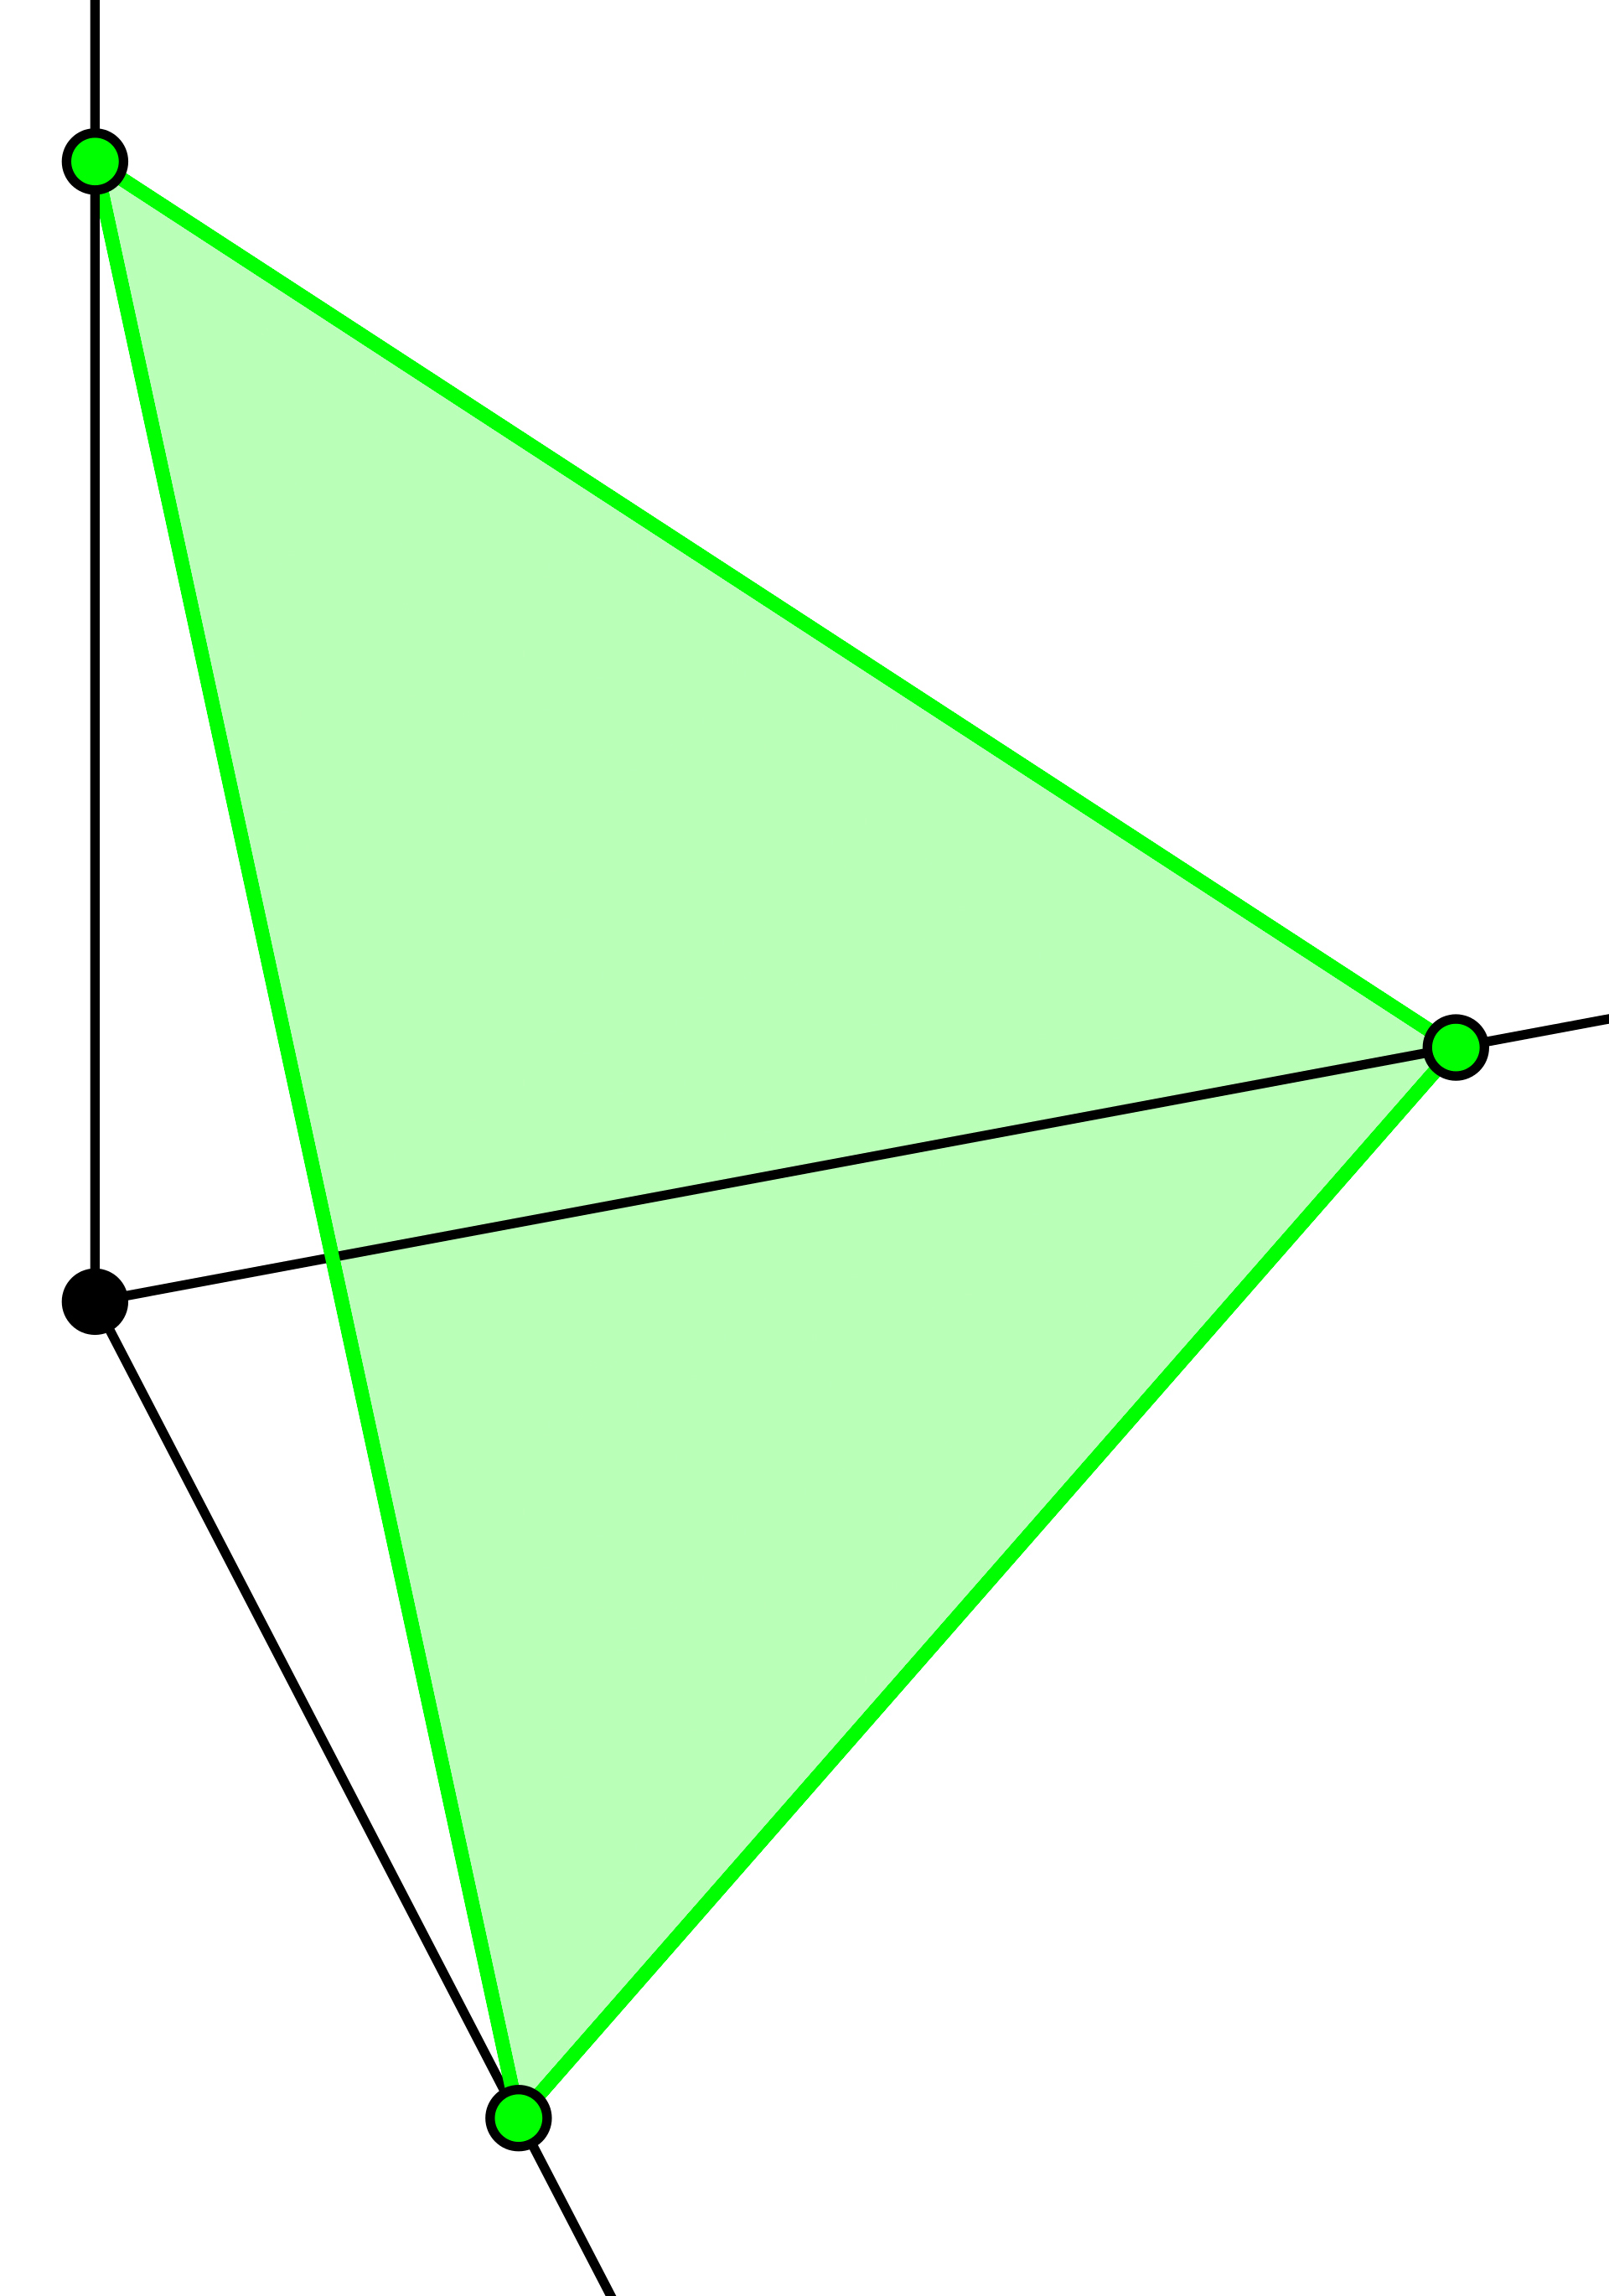
\includegraphics[scale=0.08]{2-simplex.jpg}
\vspace{-.15in}
\caption{\href{https://en.wikipedia.org/wiki/Simplex}{https://en.wikipedia.org/wiki/Simplex}よりstandard 2-simplexの図}
\label{}
\end{center}
\end{figure}
\end{frame}

\begin{frame}
\begin{center}
\animategraphics[loop,controls,width=.5\linewidth]{5}{dirichlet-}{0}{15}
\href{https://medium.com/@lettier/how-does-lda-work-ill-explain-using-emoji-108abf40fa7d}{{\scriptsize https://medium.com/@lettier/how-does-lda-work-ill-explain-using-emoji-108abf40fa7d}}
\end{center}
\end{frame}

\begin{frame}{ガンマ関数}
\begin{itemize}
\item ガンマ関数について次の等式が成り立つ
\begin{align}
\Gamma(x+1)=x\Gamma(x) 
\label{eq:gamma}
\end{align}
\item この授業でガンマ関数について把握すべきことは式\eqref{eq:gamma}だけ
\item 上式より、自然数$n$について、$\Gamma(n+1)=n!$
\begin{itemize}
\item 式\eqref{eq:gamma}はガンマ関数の定義から導かれるが、定義は知らなくてよい
\item ガンマ関数は実際は複素数について定義されるが、ここでは実数、しかも正の実数を引数とする場合しか扱わない
\item ディリクレ分布の規格化定数が$\frac{\Gamma(\sum_{w=1}^W \beta_w)}{\prod_{w=1}^W\Gamma(\beta_w)}$である証明は割愛する
\begin{itemize}
\item[cf.] {\scriptsize \href{https://faculty.math.illinois.edu/\~r-ash/Stat/StatLec1-5.pdf}{\url{https://faculty.math.illinois.edu/~r-ash/Stat/StatLec1-5.pdf}}のSec.~5.4}
\end{itemize}
\end{itemize}
\end{itemize}
\end{frame}

\begin{frame}
\begin{figure}[htbp]
\begin{center}
\includegraphics[scale=0.4]{650px-Gamma_plot.svg}
\caption{\href{https://en.wikipedia.org/wiki/Gamma_function}{ガンマ関数}}
\label{}
\end{center}
\end{figure}
\end{frame}

\begin{frame}{ベータ分布とディリクレ分布}
\begin{itemize}
\item ベータ分布は、ディリクレ分布で$W=2$の場合に対応する
\item アイテムの種類が2種類の場合と3種類以上の場合との対応関係は、以下の表のとおり
\end{itemize}
\begin{table}
\begin{center}
\begin{tabular}{|c|c|}
\hline アイテムが2種類の場合 & アイテムが3種類以上の場合 \\ \hline
ベルヌーイ分布 & カテゴリカル分布 \\
二項分布 & 多項分布 \\
ベータ分布 & ディリクレ分布 \\ \hline
\end{tabular}
\end{center}
\end{table}
\end{frame}

\begin{frame}{ベータ分布の二項分布に対する関係 (1/2)}
\begin{itemize}
\item 「二項分布をひとつ選ぶこと」=「$\phi_1$の値を選ぶこと」
\end{itemize}
\begin{figure}[t]
\begin{center}
\includegraphics[scale=0.13]{beta1.png}
\end{center}
\end{figure}
\end{frame}

\begin{frame}{ベータ分布の二項分布に対する関係 (2/2)}
\begin{itemize}
\item 「二項分布をひとつ選ぶこと」=「$[0,1]$上の1点を選ぶこと」
\end{itemize}
\begin{figure}[t]
\begin{center}
\includegraphics[scale=0.13]{beta2.png}
\end{center}
\end{figure}
\end{frame}

\begin{frame}
\begin{figure}[htbp]
\begin{center}
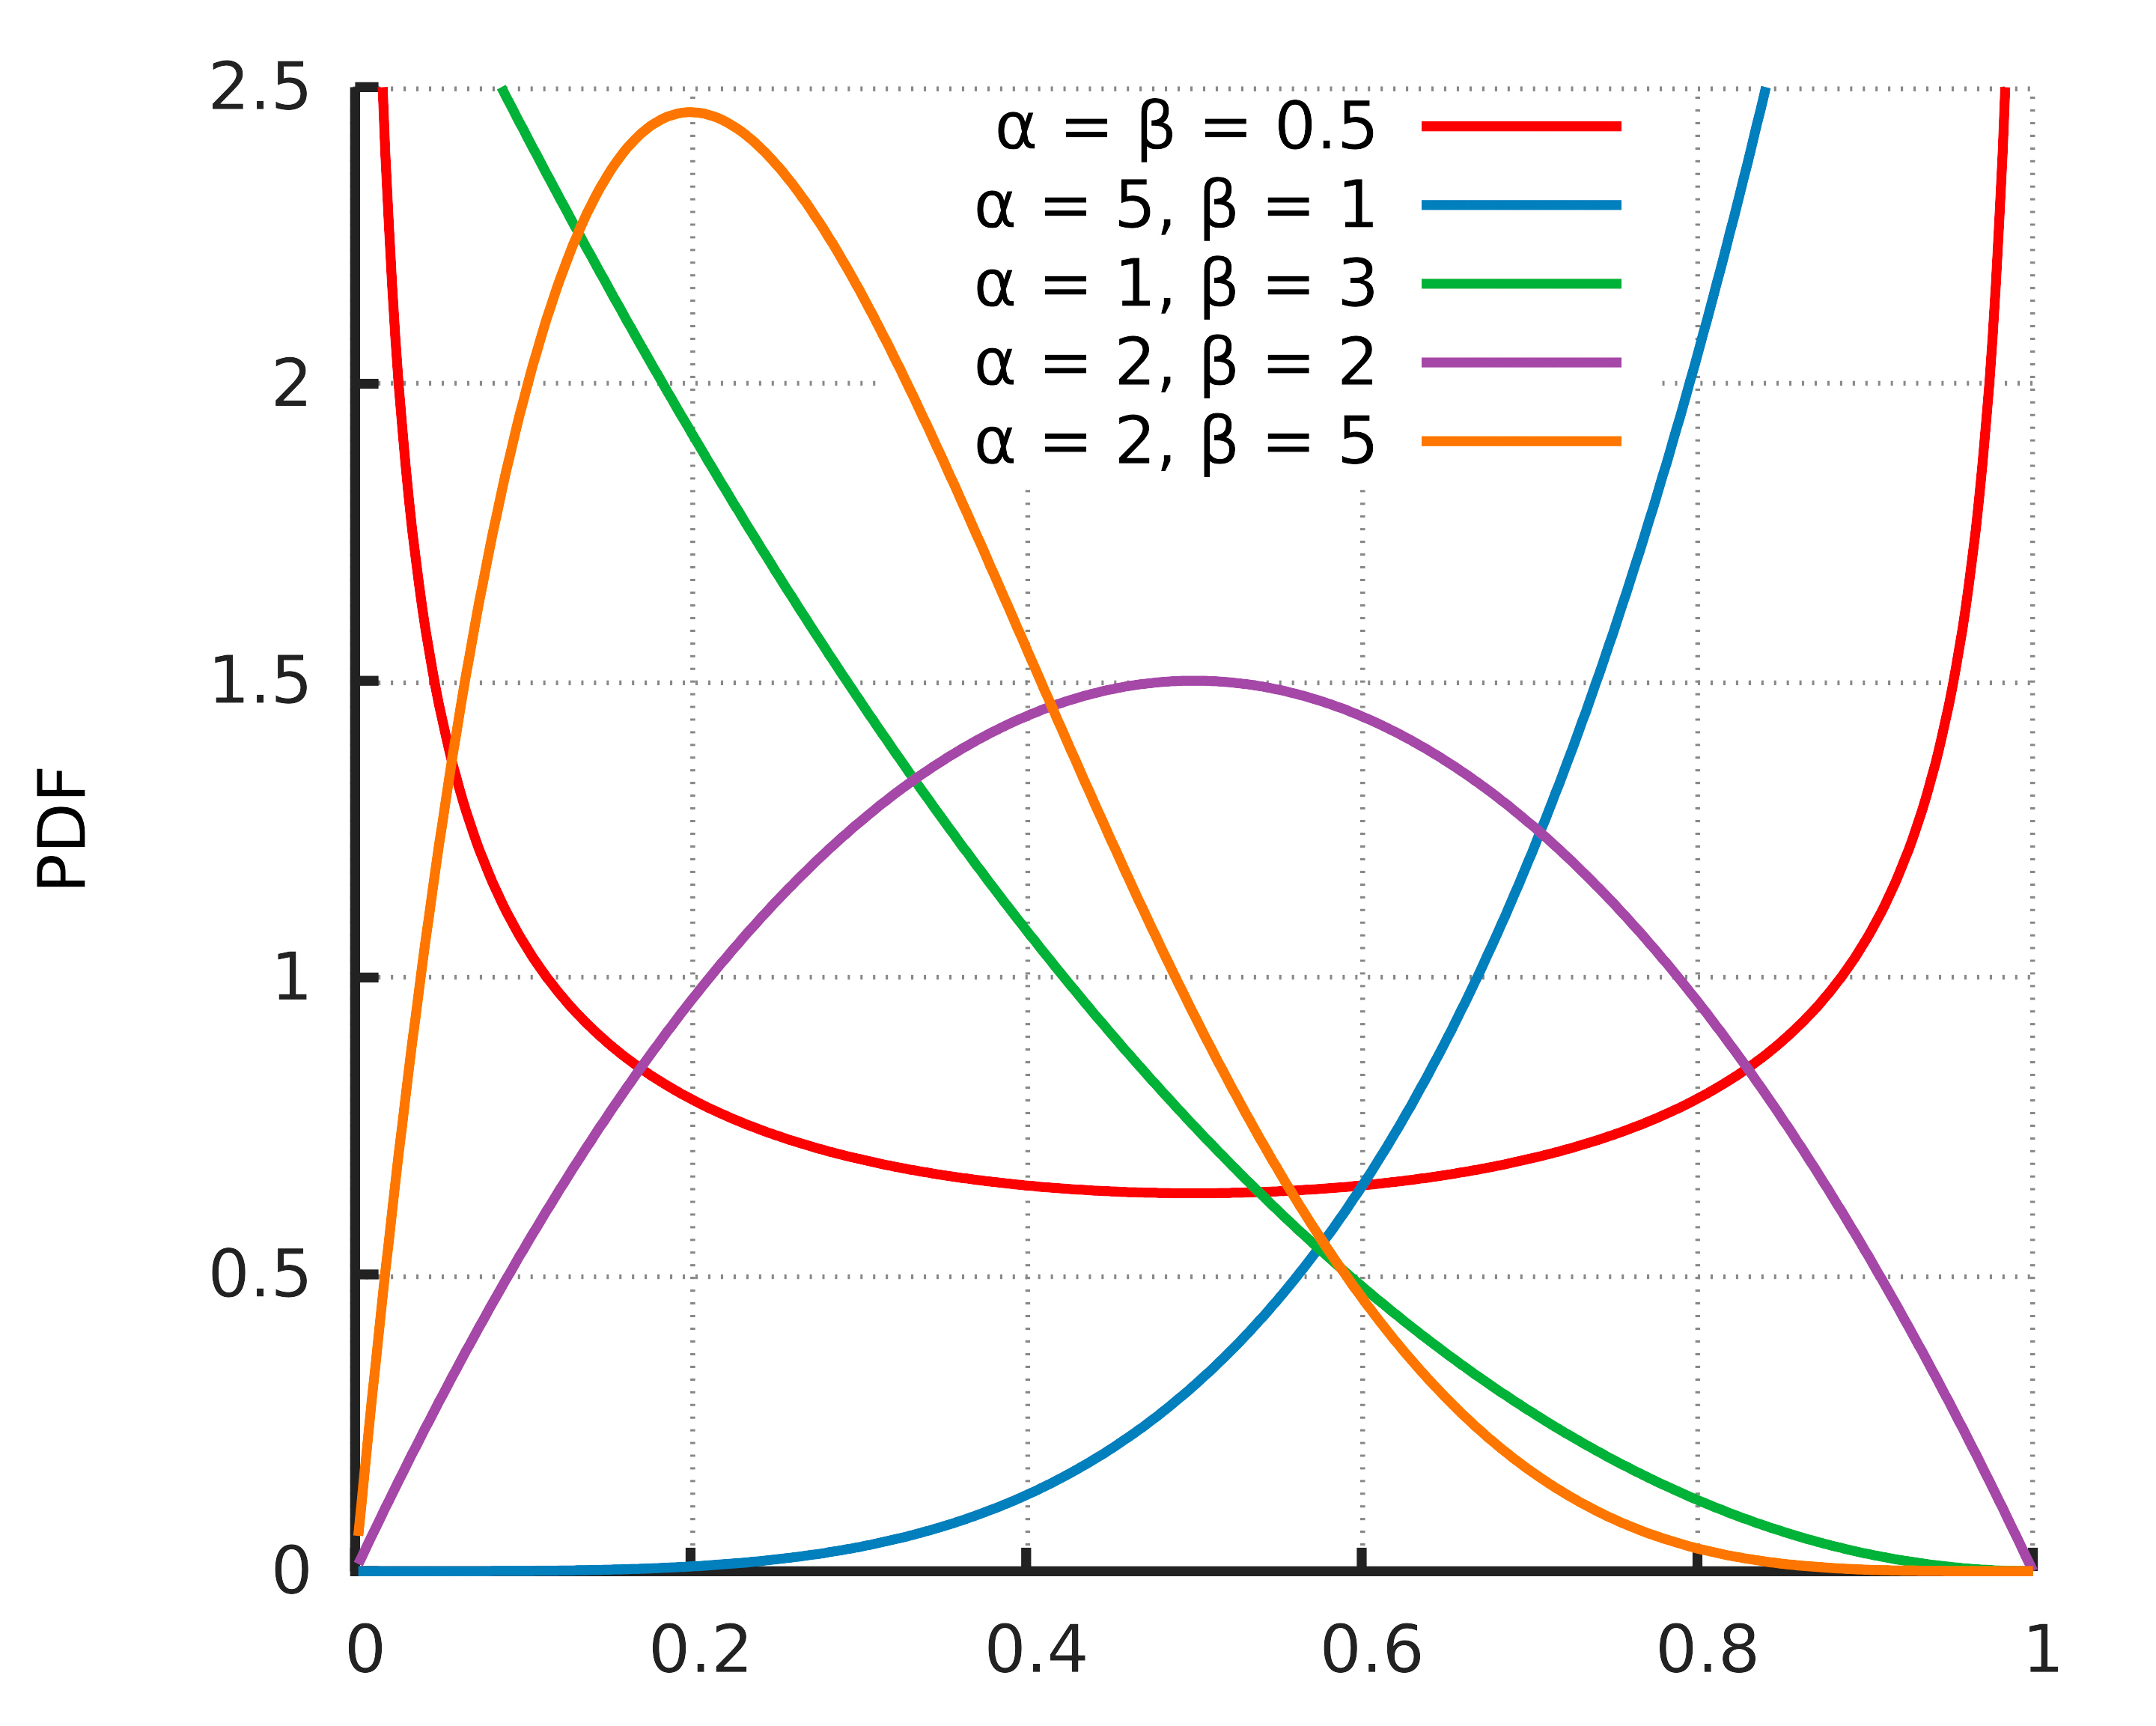
\includegraphics[scale=0.09]{beta-distribution.jpg}
\vspace{-.2in}
\caption{\href{https://en.wikipedia.org/wiki/Beta_distribution}{https://en.wikipedia.org/wiki/Beta\_distribution}}
\label{}
\end{center}
\end{figure}
\end{frame}

\begin{frame}{分布の分布としてのベータ分布}
\begin{itemize}
\item ベータ分布は$[0,1]$($1$次元単体)の上に定義される
\item $[0,1]$上の一点一点が、別々の二項分布に対応している
\begin{itemize}
\item[例.] $0.6\in[0,1]$は$\bm{\phi}=(0.6,0.4)$をパラメータとする二項分布に対応
\item 2つのパラメータのうち一方を決めると他方は自動的に決まる
\item ただし、試行の総数$n$はあらかじめ固定されているとする
\end{itemize}
\item ということは、ベータ分布は二項分布の集合上に定義された分布とみなせる
\begin{itemize}
\item つまり、ベータ分布は、分布の分布とみなせる
\end{itemize}
\end{itemize}
\end{frame}

\begin{frame}{分布の分布としてのディリクレ分布}
\begin{itemize}
\item ディリクレ分布は$W-1$次元単体の上に定義される
\begin{itemize}
\item 1次元単体は線分、2次元単体は正三角形、3次元単体は正四面体
\end{itemize}
\item $W-1$次元単体の一点一点が別々の多項分布に対応している
\begin{itemize}
\item 多項分布の$W$個のパラメータ$\bm{\phi}=(\phi_1,\ldots,\phi_W)$のうち$W-1$個、例えば$\phi_1$から$\phi_{W-1}$を決めると、残り1個は決まる
\item よって多項分布のパラメータ$\bm{\phi}=(\phi_1,\ldots,\phi_W)$の取りうる値の組のひとつひとつが、$W-1$次元単体に含まれる1点1点に対応
\end{itemize}
\item ということは、ディリクレ分布は多項分布の集合上に定義された分布とみなせる
\begin{itemize}
\item つまり、ディリクレ分布は、分布の分布とみなせる
\end{itemize}
\end{itemize}
\end{frame}

\begin{frame}{多項分布を使うベイズ的モデルの``部品''}
\begin{itemize}
\item $p(\bm{x}|\bm{\phi})$ 観測データ$\bm{x}=\{x_1,\ldots,x_n\}$の尤度
\begin{itemize}
\item $x_i$は$i$番目に出現するアイテムを表す確率変数
\item 事前分布を使わないときは$p(\bm{x};\bm{\phi})$と書いていた
\item ベイズ的モデリングでは、$p(\bm{x}|\bm{\phi})$と、条件付き確率として書く
\item これは、観測変数$x_i$だけでなく、$\bm{\phi}$も確率変数となるからである
\end{itemize}
\item $p(\bm{\phi};\bm{\beta})$ 多項分布のパラメータ$\bm{\phi}$が従う事前分布
\begin{itemize}
\item $\bm{\beta}$は事前分布のパラメータ
\item 事前分布のパラメータを一般にハイパーパラメータと呼ぶ
\item ・・・というわけで、ここにディリクレ分布を使うことにする
\end{itemize}
\end{itemize}
\end{frame}

\begin{frame}{事後分布 posterior distribution}
\vspace{-.2in}
\begin{align}
p(\bm{\phi}|\bm{x};\bm{\beta}) \propto p(\bm{x}|\bm{\phi})p(\bm{\phi};\bm{\beta})
\label{eq:bayes_posterior}
\end{align}
\vspace{-.2in}
\begin{itemize}
\item ベイズ的モデリングは、事後分布を求めることを課題とする
\item 事後分布はモデルパラメータ$\bm{\phi}$が従う確率分布で、観測データ$\bm{x}$が所与の条件付き確率分布
\item 事後分布は、式\eqref{eq:bayes_posterior}のように、ベイズ則によって観測データの尤度$p(\bm{x}|\bm{\phi})$と事前分布$p(\bm{\phi};\bm{\beta})$とから導き出される
\begin{itemize}
\item 事後分布$p(\bm{\phi}|\bm{x};\bm{\beta})$は、パラメータが取りうる値の全てについて、それぞれがどのくらいありえそうかを表している
\end{itemize}
\end{itemize}
\end{frame}

\begin{frame}{事後分布を求めることと最尤推定との一つの違い}
\begin{itemize}
\item 最尤推定は、データ尤度$p(\bm{x}|\bm{\phi})$をパラメータ$\bm{\phi}$の関数とみなして最大化することで、$\bm{\phi}$の値をひとつに決める
\begin{align}
\argmax_{\bm{\phi}} p(\bm{x}|\bm{\phi})
\notag
\end{align}
\item 一方、ベイズ的なモデリングでは、パラメータ$\bm{\phi}$が取りうる全ての値について、各々どのくらいありえそうかを表している事後分布$p(\bm{\phi}|\bm{x};\bm{\beta})$を、求める
\begin{align}
p(\bm{\phi}|\bm{x};\bm{\beta}) \propto p(\bm{x}|\bm{\phi})p(\bm{\phi};\bm{\beta})
\notag
\end{align}
\end{itemize}
\end{frame}

\begin{frame}{事後分布の直感的な意味}
\vspace{-.2in}
\begin{align}
p(\bm{\phi}|\bm{x};\bm{\beta}) \propto p(\bm{x}|\bm{\phi})p(\bm{\phi};\bm{\beta})
\end{align}
\vspace{-.2in}
\begin{itemize}
\item 上の式は、事前分布$p(\bm{\phi};\bm{\beta})$が尤度$p(\bm{x}|\bm{\phi})$によって重み付けし直されて事後分布になる、という式
\item $\bm{\phi}$が尤度$p(\bm{x}|\bm{\phi})$を大きくするような値だと、右辺においてそれだけ大きな値が掛け算される
\item よって、左辺の事後分布で$\bm{\phi}$がそのような値を取る確率は大
\end{itemize}
\end{frame}

\begin{frame}{共役事前分布 conjugate prior distribution}
\begin{itemize}
\item 共役事前分布とは、事後分布を事前分布と同じ種類の分布にするような事前分布のことをいう
\item 例えば、データ尤度$p(\bm{x}|\bm{\phi})$が多項分布で表されているとき、
事前分布としてディリクレ分布を用いると、事後分布もディリクレ分布となる
\item つまり、ディリクレ分布は共役事前分布である
\item このため、多項分布を使ってベイズ的なモデリングをするとき、ディリクレ分布を事前分布に使うことが多い
\begin{itemize}
\item ディリクレ分布以外の分布を事前分布として使うこともある
\item 例えば、logit-normal distributionを使うことがある
\end{itemize}
\end{itemize}
\end{frame}

\begin{frame}{問題5-1}
\large
\begin{itemize}
\item ディリクレ分布が共役事前分布であることを示せ
\item ヒント:尤度が多項分布を使って表されるとき、事前分布をディリクレ分布にすると、事後分布もディリクレ分布になることを示せばよい
\end{itemize}
\end{frame}

\begin{frame}
\FontMath
\begin{align}
p(\bm{x}|\bm{\phi})p(\bm{\phi};\bm{\beta})
& =
\frac{n!}{\prod_w c_w!} \prod_w \phi_w^{c_w} \times \frac{\Gamma(\sum_w \beta_w)}{\prod_w \Gamma(\beta_w)}\prod_w \phi^{\beta_w - 1}
\propto
\prod_w \phi_w^{c_w + \beta_w - 1}
\end{align}
$p(\bm{\phi}|\bm{x};\bm{\beta}) \propto p(\bm{x}|\bm{\phi})p(\bm{\phi};\bm{\beta})$より、
\begin{align}
p(\bm{\phi} | \bm{x}; \bm{\beta}) \propto \prod_w \phi_w^{c_w + \beta_w - 1}
\end{align}
あとは、規格化定数normalizing constantを求めればよい。
\begin{align}
\int_{\{ \bm{\phi}: \sum_w \phi_w = 1 \}} \prod_w \phi_w^{c_w + \beta_w - 1} d\bm{\phi} 
= \frac{\prod_w \Gamma(c_w+\beta_w)}{\Gamma(n + \sum_w \beta_w)}
\end{align}
よって、
\begin{align}
p(\bm{\phi} | \bm{x}; \bm{\beta}) = \frac{\Gamma(n + \sum_w \beta_w)}{\prod_w \Gamma(c_w+\beta_w)}
\prod_w \phi_w^{c_w + \beta_w - 1}
\end{align}
\end{frame}

\begin{frame}{最大事後確率推定(MAP推定)}
\begin{itemize}
\item 事後確率を最大化する$\bm{\phi}$の値をモデルパラメータの推定値とする推定方法を、最大事後確率推定という
\begin{align}
\hat{\bm{\phi}}_{\mbox{\scriptsize MAP}} = \argmax_{\bm{\phi}} p(\bm{\phi}|\bm{x};\bm{\beta})
\end{align}
\begin{itemize}
\item MAP推定と略される(MAP; maximum a posteriori)
\end{itemize}
\item 下記の最尤推定と同様、モデルパラメータ$\bm{\phi}$の値をひとつ選ぶ推定方法
\begin{align}
\hat{\bm{\phi}}_{\mbox{\scriptsize ML}} = \argmax_{\bm{\phi}} p(\bm{x};\bm{\phi})
\end{align}
\end{itemize}
\end{frame}

\begin{frame}{多項分布のMAP推定}
\begin{itemize}
\item 観測データのモデルが多項分布で、ディリクレ分布が事前分布のとき、MAP推定が与える解は
\begin{align}
\hat{\phi}_w = \frac{c_w + \beta_w - 1}{\sum_w (c_w + \beta_w - 1)} 
\end{align}
\begin{itemize}
\item 問:なぜこうなるか、示せ
\end{itemize}
\item アイテムの実際の出現頻度ではなく、$\beta_w - 1$回だけ下駄を履かせた出現頻度で確率を計算していることになる
\begin{itemize}
\item 単語の出現確率を求めるとき、このように下駄を履かせた回数を代わりに使うことを、スムージングsmoothingという
\end{itemize}
\end{itemize}
\end{frame}


\section{多項分布のMAP推定の応用}

\begin{frame}\frametitle{Contents}
\Large \tableofcontents[currentsection]
\end{frame}

\begin{frame}{情報検索 information retrieval}
\begin{itemize}
\item たくさんの文書を持っている
\item それらの文書をクエリに適合する(relevantな)順にソート
\begin{itemize}
\item 情報検索とは、このようなことをすること
\end{itemize}
\item どう実装すればいい?
\item 実装例
\begin{itemize}
\item ひとつひとつの文書について別々に単語出現確率$\bm{\phi}$を\underline{MAP推定}
\item 推定された$\bm{\phi}$を使って、クエリの生成確率を計算
\item この生成確率を高くする順に文書をソート
\end{itemize}
\end{itemize}
\end{frame}

\begin{frame}{文書をランキングするための計算}
\begin{itemize}
\item 上述のMAP推定は、検索対象の文書群のうち$d$番目の文書について単語$\mbox{v}_w$の出現確率を
$\hat{\phi}_{d,w} = \frac{c_{d,w} + \beta_w - 1}{\sum_w (c_{d,w} + \beta_w - 1)}$と与える
\begin{itemize}
\item たとえ$\mbox{v}_w$が文書$d$に現れない単語であっても、つまり$c_{d,w}=0$であっても、$\beta_w > 1$ならば確率がゼロにならないことに注意
\end{itemize}
\item この単語確率によってクエリ$\bm{x}_q$が生成される確率は:
\begin{align}
p(\bm{x}_q | \hat{\phi}_d) = \frac{n_q!}{\prod_w c_{q,w}!}
\prod_w \bigg( \frac{c_{d,w} + \beta_w - 1}{\sum_w (c_{d,w} + \beta_w - 1)} \bigg)^{c_{q,w}}
\end{align}
\begin{itemize}
\item $c_{q,w}$はクエリにおける単語$\mbox{v}_w$の出現頻度
\end{itemize}
\item $p(\bm{x}_q | \hat{\phi}_d)$の降順に、文書をソートすればよい
\end{itemize}
\end{frame}

\begin{frame}
\begin{figure}[htbp]
\begin{center}
\includegraphics[scale=0.42]{IR_MAP.png}
\label{}
\end{center}
\end{figure}
\end{frame}

\begin{frame}{背景確率を使ったスムージング}
\begin{itemize}
\item MAP推定によると$d$番目の文書における単語$\mbox{v}_w$の出現確率は
$\hat{\phi}_{d,w} = \frac{c_{d,w} + \beta_w - 1}{\sum_w (c_{d,w} + \beta_w - 1)}$である
\item 実際には、コーパス全体における単語$\mbox{v}_w$の出現確率$p_w$を使って、
$\beta_w - 1$の部分を$\lambda p_w$で置き換えることが多い
\begin{itemize}
\item $p_w$のことを背景確率background probabilityと呼んだりする
\end{itemize}
\item つまり、
$\hat{\phi}_{d,w} = \frac{c_{d,w} + \lambda p_w}{c_d + \lambda}$とする
\begin{itemize}
\item $c_d \equiv \sum_w c_{d,w}$は$d$番目の文書の長さ
\end{itemize}
\item $\lambda$は検証用クエリの検索性能を見ながらチューニングする
\begin{itemize}
\item[cf.] \href{https://nlp.stanford.edu/IR-book/html/htmledition/estimating-the-query-generation-probability-1.html}{{\tiny https://nlp.stanford.edu/IR-book/html/htmledition/estimating-the-query-generation-probability-1.html}} 
\end{itemize}
\end{itemize}
\end{frame}

\end{document}